\documentclass[../EngineeringJournal_CDavis.tex]{subfiles}

\begin{document}

%%%%%%%%%%%%%%%%%%%%%%%%%%%%%%%%%%%%%%%%%%%%%%%%%%%%%
%%%%%%%%%%%%%%%%%%%%%%%%%%%%%%%%%%%%%%%%%%%%%%%%%%%%%

\chapter[Configuring IPv6 Static Routes]{Configuring IPv6 \linebreak[1] Static Routes \hspace*{\fill}{Feb 6, 2020}}
\noindent\textbf{{Packet Tracer Lab 5} \hspace*{\fill}{\textbf{CIT 167}}}\linebreak[1]
{{Spring 2020} \hspace*{\fill}{Chaz Davis}}                             
%===================================
%===================================

\hspace{0.2cm}
\begin{tcolorbox}[width=6.3in]
\scriptsize 
- Important Commands for the Lab
  \begin{itemize}
    \item{ipv6 unicast-routing}
    \item{ipv6 route} 
    \item{show ipv6 interface brief} 
  \end{itemize}
\normalsize
- Important notes about IPv6
\scriptsize
\\IPv6 uses a new mechanism for mapping IP addresses to link layer addresses 
(MAC addresses), because it does not support the broadcast addressing method, 
on which the functionality of the Address Resolution Protocol (ARP) in IPv4 is based. 
IPv6 implements the Neighbor Discovery Protocol (NDP, ND) in the link layer, 
which relies on ICMPv6 and multicast transmission. IPv6 hosts verify the 
uniqueness of their IPv6 addresses in a local area network (LAN) 
by sending a neighbor solicitation message asking for the link layer 
address of the IP address. If any other host in the LAN is 
using that address, it responds.
\normalsize
\end{tcolorbox}
\hspace{0.2cm}

\newpage

%===================================
\mysection{\textbf{Part 1:Examine the Network}}
\mysubsection{1}{a}\\
There are 5 networks connected in the current topology

\begin{figure}[!hbt]
  \centering
  \subfloat[Topology]{\label{Top5a}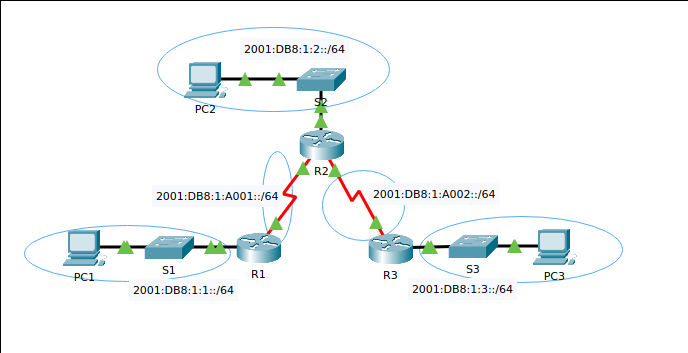
\includegraphics[width=.45\linewidth]{Figures/2020-02-04-104354_688x353_scrot.png}}
  \caption{Topology of the Network}\label{Top5}
\end{figure}

\noindent\mysubsection{2}{b}\\
In Fig~\ref{Top5} we can see the R1 and R3 each have two connected networks, and that R2 has three connected networks.

\noindent\mysubsection{3}{c}\\
Ipv6 route then we specify [the network, and  prefix] then we specify either [next hop address or exit interface]

%===================================
\mysection{\textbf{Part 2: Configure IPv6 static and default routes}}

\mysubsection{1}{Enabling the Routers}\\
I logged into Each of the routers ena, conf t, and then typed 
in {\scriptsize{\verb$ipv6 unicast-routing$}\normalsize} into each terminal as seen in Fig~\ref{Enable5V6}.

\begin{figure}[!hbt]\centering
\subfloat[R1 Enable]{\label{Enable5V6R1}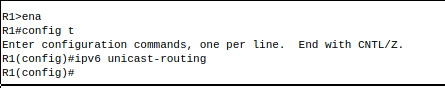
\includegraphics[width=.45\linewidth]{Figures/2020-02-04-105919_445x88_scrot.png}}\hfill
\subfloat[R2 Enable]{\label{Enable5V6R2}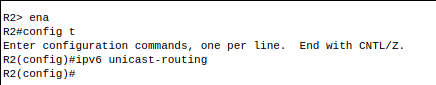
\includegraphics[width=.45\linewidth]{Figures/2020-02-04-105934_436x85_scrot.png}}\par 
\subfloat[R3 Enable]{\label{Enable5V6R3}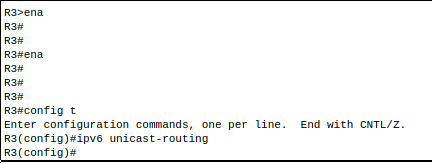
\includegraphics[width=.45\linewidth]{Figures/2020-02-04-105906_432x163_scrot.png}}
\caption{Enabling IPv6}\label{Enable5V6}
\end{figure}

\clearpage

\noindent\mysubsection{2}{Configuring the routers}\\
Next I went to the three routers and manually entered the info for the network
configuring each destination and each hop on the network. See Fig~\ref{IPv6Rman5}.

\begin{figure}[!hbt]\centering
\subfloat[Manually entering the network info on R1]{\label{IPv6man5R1}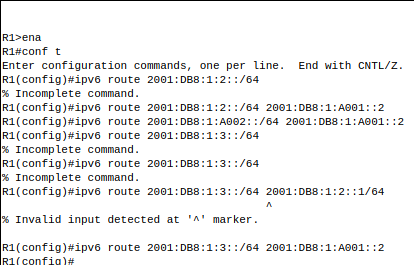
\includegraphics[width=.40\linewidth]{Figures/2020-02-05-133704_414x265_scrot.png}}\hfill
\subfloat[Manually entering the network info on R2]{\label{IPv6man5R2}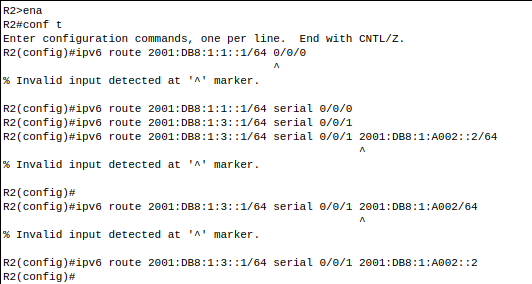
\includegraphics[width=.46\linewidth]{Figures/2020-02-05-134344_532x284_scrot.png}}\par 
\subfloat[Manually entering the network info on R3]{\label{IPv6man5R3}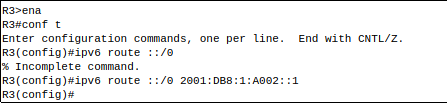
\includegraphics[width=.45\linewidth]{Figures/2020-02-05-134521_447x103_scrot.png}}
\caption{Manually Configuring the Destination IPv6 address, as well as the next hop address and Exit address}\label{IPv6Rman5}
\end{figure}

\clearpage

\noindent\mysubsection{3}{Verifying Static Route Configurations}\\

\begin{figure}[!hbt]\centering
\subfloat[IPv6Config]{\label{ipv65config}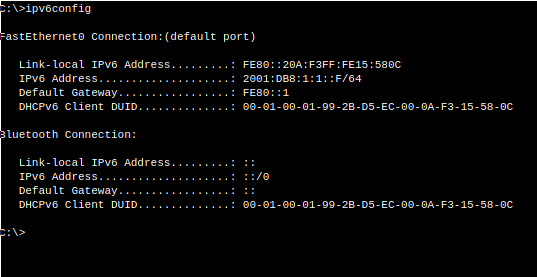
\includegraphics[width=.45\linewidth]{Figures/2020-02-05-141628_537x277_scrot.png}}\par
\subfloat[IPv6 Interface brief]{\label{ipv65intbrief}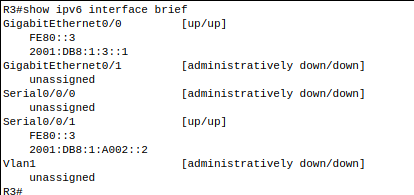
\includegraphics[width=.45\linewidth]{Figures/2020-02-05-141722_414x195_scrot.png}}\hfill 
\subfloat[show ipv6 route]{\label{ipv65route}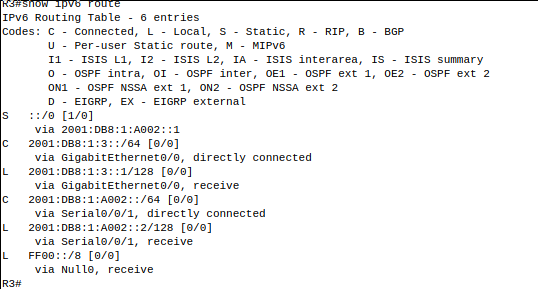
\includegraphics[width=.45\linewidth]{Figures/2020-02-05-141748_538x289_scrot.png}}
\caption{Verifying the Network}\label{IPv65ver}
\end{figure}

\subsubsection{a}{PC command}\\
From the command prompt in the PC terminals, I entered
the command {\scriptsize{\verb$ipv6 config$}\normalsize} for information on the network See
Fig~\ref{IPv65ver}\subref{ipv65config}

\subsubsection{b}{routing address}\\
From the routers terminals 
I entered {\scriptsize{\verb$show ipv6 interface brief$}\normalsize}  to display 
the configured addresses. See Fig~\ref{IPv65ver}\subref{ipv65intbrief}

\subsubsection{c}{Routing Table}\\
Finally, I entered {\scriptsize{\verb$Show ipv6 route$}\normalsize} into each of the 
prompts to display the routing tables. See Fig~\ref{IPv65ver}\subref{ipv65route}

\clearpage

%===================================
\mysection{\textbf{Part 3: Success}}
\begin{center}
	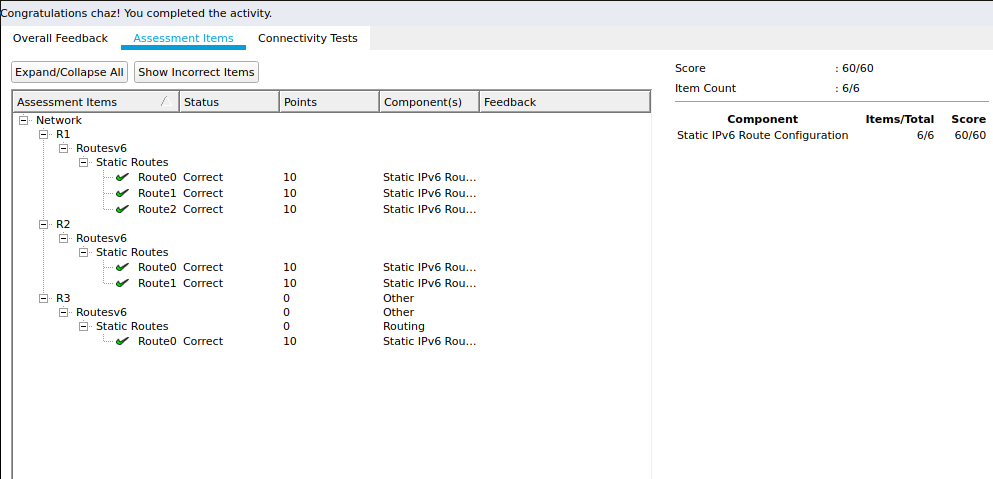
\includegraphics[scale=0.25]{Figures/2020-02-05-141927_993x479_scrot.png}
\end{center}

%===================================
\end{document}
